\newcommand{\figureSoundGraph}[1]{
  \begin{figure}[H]
    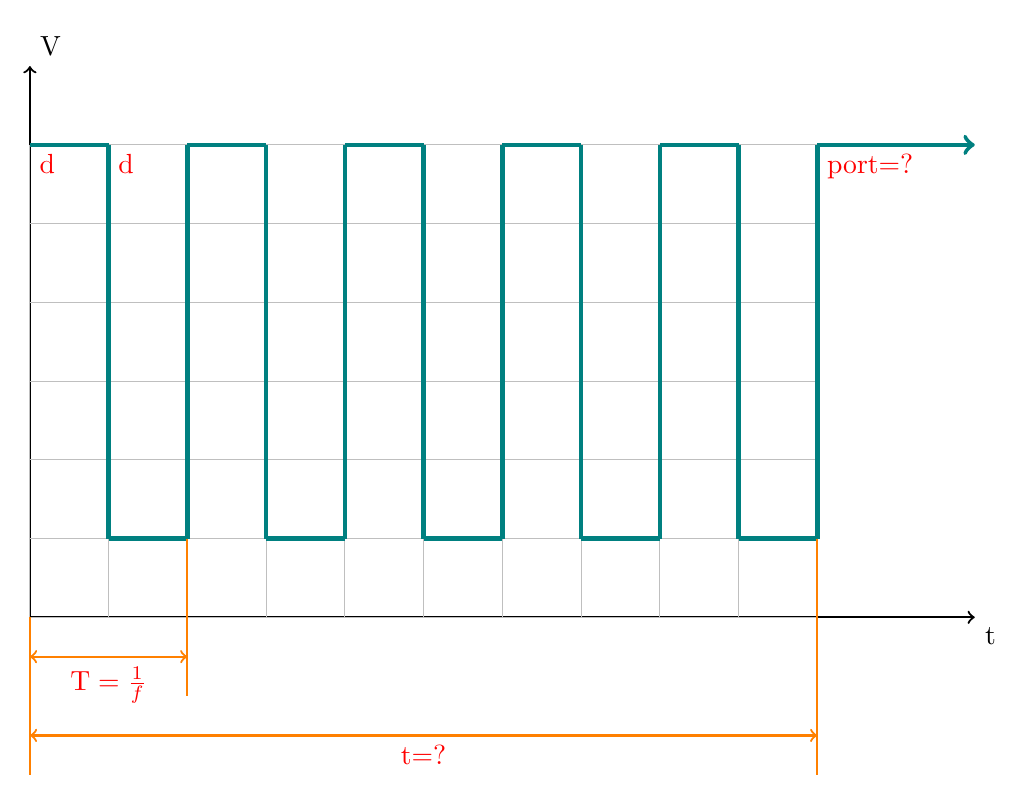
\begin{tikzpicture}
      \draw[thick, ->] (0, 0) -- (12, 0) node[anchor=north west] {t};
      \draw[thick, ->] (0, 0) -- (0,  7) node[anchor=south west] {V};
      \draw[lightgray] (0, 0) grid (10, 6);
      \foreach \x in {0, 2, ..., 8} {
        \draw[ultra thick, teal] (\x, 6) -- (\x + 1, 6);
        \draw[ultra thick, teal] (\x + 1, 6) -- (\x + 1, 1);
        \draw[ultra thick, teal] (\x + 1, 1) -- (\x + 2, 1);
        \draw[ultra thick, teal] (\x + 2, 1) -- (\x + 2, 6);
      }
      \draw[ultra thick, teal, ->] (10, 6) -- (12, 6);
      \draw[orange] (10, 6) node[anchor=north west, red] {port=?};
      \draw[orange] (0, 6) node[anchor=north west, red] {d};
      \draw[orange] (1, 6) node[anchor=north west, red] {d};
      \draw[thick, orange] (0,  0) -- (0,   -2);
      \draw[thick, orange] (2,  1) -- (2,   -1);
      \draw[thick, orange] (10, 1) -- (10,  -2);
      \draw[thick, orange, <->] (0, -0.5)
      -- (2,  -0.5) node[midway, below, red] {$\mbox{T} = \frac{1}{f}$};
      \draw[thick, orange, <->] (0, -1.5)
      -- (10,  -1.5) node[midway, below, red] {t=?};
    \end{tikzpicture}
    \caption{#1}
    \label{fig:sound-graph}
  \end{figure}
}
